\documentclass[12pt]{article}
\usepackage{syderpt}
\usepackage{enumitem}
\usepackage[section]{placeins}

\begin{document}

\waterlootitle{Lamprey Muscle Control with Feedback}{

}{
  Jennifer Blight  20347163\\
  4B Systems Design Engineering\\
  April 25th, 2014
  }

\pagenumbering{roman}

\onehalfspacing
\tableofcontents
\newpage
\doublespacing
\addcontentsline{toc}{section}{\listfigurename}
\listoffigures
\newpage

\pagenumbering{arabic}

\section{System Description}
The lamprey locomotion model developed by Eliasmith and Anderson \cite{Elias} demonstrates the use of the Neural Engineering Framework (NEF) in modelling complex behaviour. This model is related to the idea of a central pattern generator, a group of neurons that produces patterns of activity without sensory input. The model works by solving for optimal high-level control signals based on orthogonal basis functions and then projects them onto localized groups of neurons. The resulting "muscles" can be shown to exhibit realistic oscillatory behaviour.   

While the original model is designed to operate without input, we would like to consider a situation in which motor behaviour is controlled based on some error signal. This could serve as a model for more conciously controlled behaviour and potentially be applied to designing neural control systems. Ideally, it should also rid us of the need to pre-determine the local activities, allowing us to implement specific behaviour with less analysis.

There is some question as to what constitutes a realistic and effective control signal. As with the original model, we might consider either high-level or low-level behaviour. At a high level, we might be interested in matching a target speed while also maximizing efficiency. At a lower level, we might be interested in matching a known position function. The former, high-level goals are more difficult to relate to individual muscle control but could conceivably play a role in motor learning. The latter assumes a much more specific target and modulates the control signal to meet it, perhaps more similar to the role of the cerebellum, modulating voluntary movement based on proprioception, and certainly similar to modern control systems. 

This report focuses on this lower level control implementation. The goal is to set up a recurrent relation in which the muscle activity is determined based on a "proprioception" signal and a target trajectory. The system will consist mainly of the local activity signals used in the original lamprey locomotion model and the corresponding muscle tensions. The muscle tensions are used as a proprioception signal rather than relative position as they produce a similar signal without requiring the construction of a physical simulation of the lamprey. Two different approaches are considered: one using a direct negative feedback loop and another which attempts to learn a recurrent relation. These are compared to the original model.

\newpage
\section{Design Specification}

The system is largely similar to the original model. We assume a lamprey constructed of ten simplified vertebrae, each with two opposing muscles. Similarly, the target tension is defined by the equation:
\begin{equation}
  T(z,t) = \kappa (\sin(\omega t - kz) - \sin(\omega t))
\end{equation} 
where \(\kappa = \frac{\gamma \eta \omega A L }{2\pi}\) is a scaling factor and parameters \(A\), \(\eta\), \(\gamma\), and \(L\) are equal to 1. 

The actual tension for each segment is defined as:
\begin{equation}
  T(z,t) = \sum_i a_i \phi_i = \kappa \sum_i a_i e^{-(z-i*dx)^2/\sigma^2}
\end{equation} 
where \(a_i\) is the segment activity and \(\phi_i\) is a Gaussian basis function centred on the corresponding segment. Segment activity is modelled for each of the ten segments and the associated Gaussion basis function describes the localized effect. Based on this summation, muscle tension is represented for points corresponding to each vertebrae over the length of the lamprey, \(z \in [0, 0.1 ... 1]\), for time \(t \geq 0\). Segment activity is represented by a population of 400 neurons with a noise variance of 0.1, while the muscle tension is calculated directly. While wave speed is variable, most experiments were performed at 10Hz. 

\newpage
\section{Implementation}

Each of the following implementations represents segment activity using a ten-dimensional population of neurons, where each dimension represents segment activity for a single segment. Encoders were chosen to be orthogonal and correspond to individual segments; each encoder take a value of 1 or -1 in only a single dimension. These should correspond to neurons in each segment on either the right or left side of the spine.Muscle tension is likewise represented as a ten-dimensional population and is modeled directly based on the segment activities and basis functions. Other populations are specific to individual implementations.

\subsection{Basic Model}

We begin with a simple implementation of the original lamprey model. In this model, the high-level activity is determined analytically and defined in terms of harmonic basis functions:
\begin{gather}
  T(z,t; A) = \kappa (A_0 + \sum_{n=1}^N A_{2n-1}(t)sin(2\pi nz) + A_{2n}(t)cos(2\pi nz)) \\
  \dot{A} = M_D A + M_I U
\end{gather} 
\(M_D\) is a dynamics matrix with cyclic behaviour.
\begin{equation}
  M_D = \begin{bmatrix} -\alpha_0 & \omega & -\alpha_0 & 0 \\ \frac{-\omega}{2} & 0 & \frac{-\omega}{2} & 0 \\ -\alpha_0 & -\omega & -\alpha_0 & 0 \\ 0 & 0 & 0 & \alpha \end{bmatrix}
\end{equation}
The startup matrix, \(M_I\), was omitted as it was found to be unnecessary for steady-state behaviour. 
A projection matrix is used to move from this high level activity space to our localized activity space based on Gaussian basis functions.
\begin{equation}
    \Gamma_nm = \int \Phi_n(z)\phi_m(z)dz 
\end{equation}
Using this, we have a dynamics equation for the localized activity space, which can be implemented by our segment activity population using a recurrent connection:
\begin{gather}
  \dot{a} = m_D a \\
  m_D = \Gamma^{+} M_D \Gamma
\end{gather} 


The resulting system exhibits reasonable oscillatory behaviour, both in the segment activity and in the muscle tensions. (Figure 1) Furthermore, analysing the weights of the recurrent connection, we can see high connectivity between neurons representing the same segment. The weights in Figure 2 are organized based on encoder, with encoders for the same segment placed next to each other; light areas correspond to high positive weight and dark areas to high negative weights. This structure is reminiscient of existing neural data. \cite{Elias}

    \begin{figure}[h!]
      \centering
      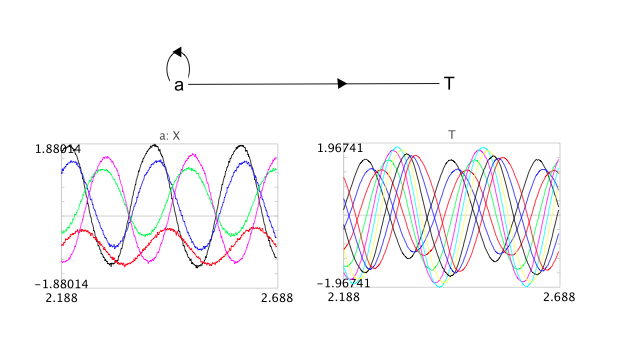
\includegraphics[scale=0.5]{neural.png}
      \caption{Output of Basic Model}
    \end{figure}

    \begin{figure}[h!]
      \centering
      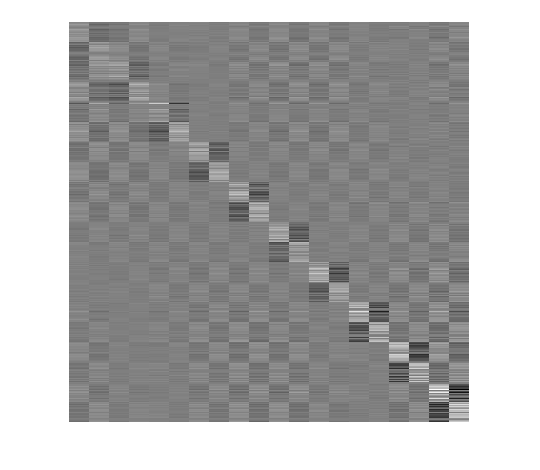
\includegraphics[scale=0.5]{fig1.png}
      \caption{Weight Matrix}
    \end{figure}

Despite a sound theoretical basis, this model was subject to a good deal of error, introduced from a variety of sources including calculating the pseudoinverse and calculating the decoders. Cyclic attractors are a degenerate case in that they require precisely competing dynamics; distortion error introduced by the decoders can destroy this behaviour by creating local attractors. 

This model is good for demonstrating the relationship between high-level and low-level dynamic representations; however, the process of generating \(m_D\) and calculating decoders may not be robust enough to error to be used in more complicated control schemes. Additionally, while the resulting weight matrix resembles actual structures, the projection from \(A\) to \(a\) is largely conceptual. In biology, the optimal recurrent relation would be learned rather than derived. Ideally, we would like to discover a similar relation via online learning. 

\subsection{Feedback Loop}
The simplest possible control model simply implements a direct negative feedback loop. A new population of 100 neurons is added to track the difference between the target tension and the actual tension. As the effects of \(a_i\) are localized, the error in tension relates to the segment activity well enough to use it as a feedback signal without any further transformations. The feedback signal modulates the segment activity. The resulting system approximates the resulting oscillations well and acheiving the correct scale is a matter of adjusting parameters such as gain. 

    \begin{figure}[h!]
      \centering
      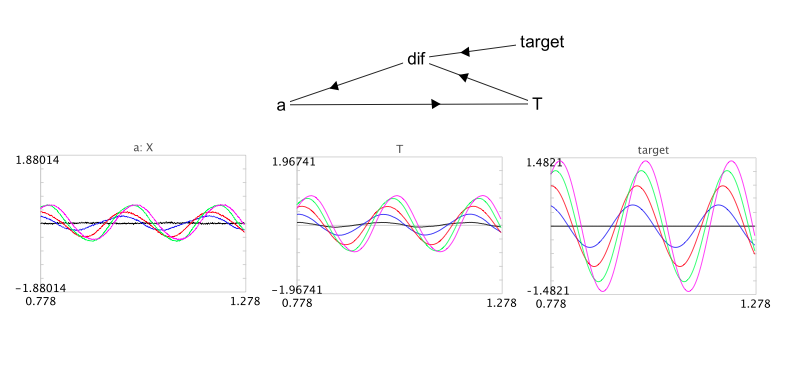
\includegraphics[scale=0.5]{feedback1.png}
      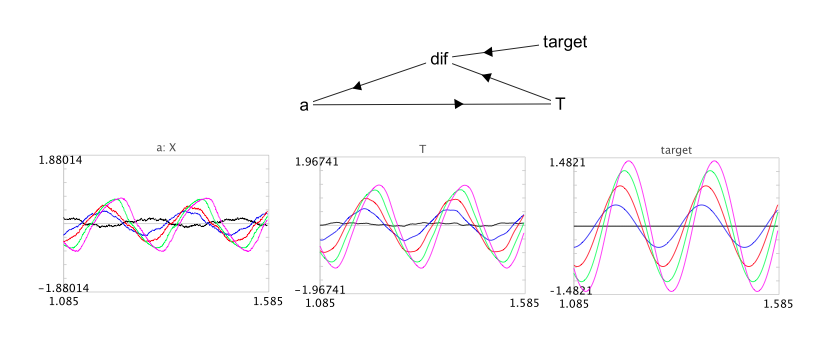
\includegraphics[scale=0.5]{feedback2.png}
      \caption[Output of Feedback Model]{Output of Feedback Model with feedback gains of 1 and 4}
    \end{figure}

This model is incredibly trivial to implement, notable only in that it is simple, works well, and appeals to standard control theory. The idea of correcting based on a target trajectory in intuitively appealing when we think about how voluntary motion might work, but this model does not have the structural link to biology that the cyclic attractor model has. Furthermore, it assumes that the intended trajectory is known in some detail, which is not necessarily the case. This is a practical approach and useful for implementing arbitrary control systems within the neural framework, but it does not necessarily reflect the biology well.

\subsection{Learned Relation}

The cyclic attractor model is compelling as a biological model but we would like to discover how such relationships arise in nature. Rather than using the error signal directly, we will attempt to learn the relationship. As usual, we will do so by adjusting the weights based on error. The error population contains 100 neurons and modifies the weights connecting the segment activity back to itself. As before, the error is based on the difference between the target tension and the actual tension. 

    \begin{figure}[h!]
      \centering
      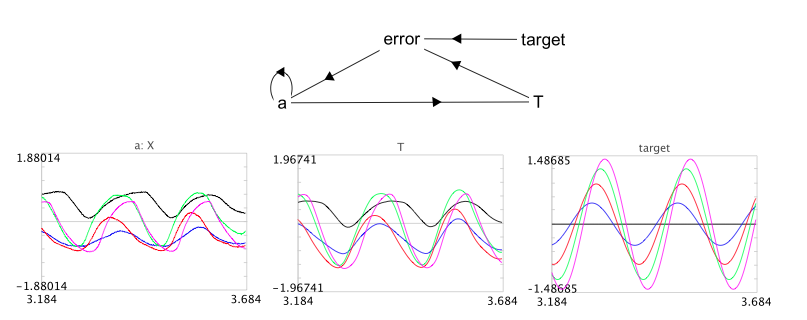
\includegraphics[scale=0.5]{learned.png}
      \caption{Output of Learned Model (Good)}
      \label{good}
    \end{figure}
    \begin{figure}[h!]
      \centering
      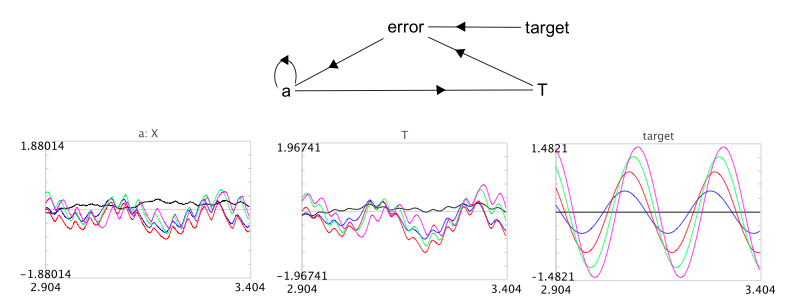
\includegraphics[scale=0.5]{fail.png}
      \caption{Output of Learned Model (Bad)}
      \label{bad}
    \end{figure}

The NEF learning framework is not well suited to learning recurrent relations. While the system can produce some oscillations (Figure \ref{good}), more often the system develops a sort of high frequency error (Figure \ref{bad}). This is likely a product of the recurrent relation. If the learning rate is high enough, the system will overcorrect for the error, because the relation is recurrent, this produces an error in the other direction which propagates again, producing an oscillation error. Adjusting the learning rate can reduce these artifacts, but also dampens the output.



Furthermore, it is worth noting that the learning rule does not produce a weight matrix similar to the one observed in the original model. The learned weight matrix varies highly in time and appears to modify all of the signals based on only a few neurons. The learned signal is highly biased towards recent data and does not generalize to the overall pattern. In this way, the learning model is really just a more complicated feedback model, one that modifies synaptic weights based on recent error rather than modifying the signal itself.

    \begin{figure}[h!]
      \centering
      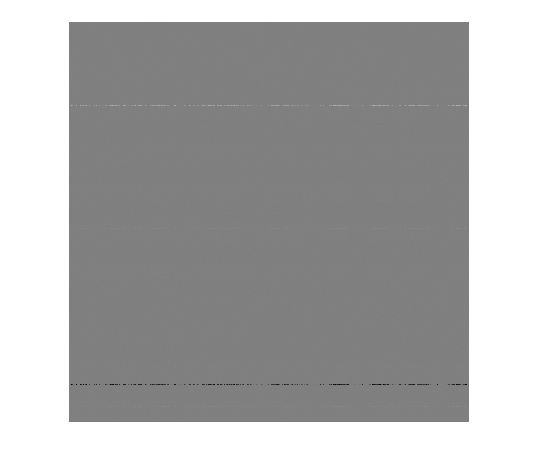
\includegraphics[scale=0.25]{fig2.png}
      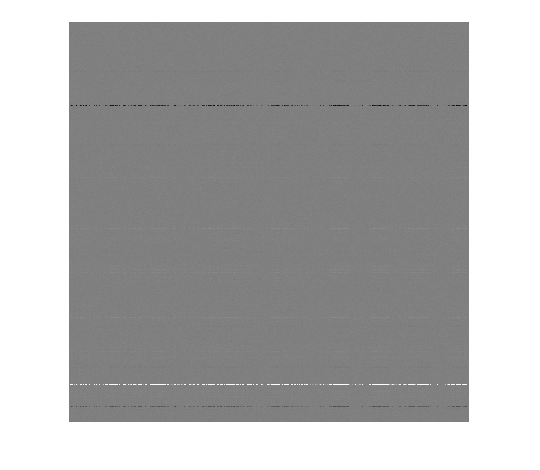
\includegraphics[scale=0.25]{fig3.png}
      \caption{Learned Weight Matrices at Different Timesteps}
    \end{figure}

Another experiment was performed in which the feedback signal was based on an ideal segment activity signal, produced by generating the correct \(A\) signal and projecting it into the intermediate level. This model performs better but is subject to the same problems with oscillating error and recency. While it is clearly more accurate to use the actual error, rather than a prozy, this model is also unrealistic in that it requires the correct activity signals in order to produce the activity signals.

    \begin{figure}[h!]
      \centering
      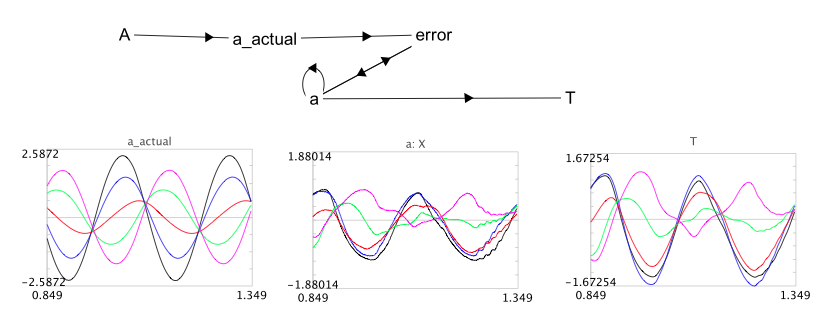
\includegraphics[scale=0.5]{learned2.png}
      \caption{Output of Learned Model}
    \end{figure}

\newpage
\section{Discussion}

We have seen thre different model for lamprey locomotion. The cyclic attractor model is biologically compelling and gives a good theoretical basis for the cyclic relationship. The feedback model is simple and practical but with no basis in biology beyond intuition. Finally, the learned model is a desirable compromise between the two, in that it tries to develop a biologically plausible model based on feedback, but fails to exhibit sufficient performance. 

Nevertheless, the learned muscle control model bears further investigation. Most motor control, for example walking and fine motor function, is learned over a period of time and eventually becomes engrained. It would be useful to have a model capable of discovering optimal relations in a similar manner. Other learning methods, including homeostatic PES, might produce different results. In particular, there are algorithms specific to real-time training of recurrent neural networks that might be useful. One might also avoid some of the problems encountered here by beginning with less cyclic behaviour, such as arm movement.

There is also a question of whether the use of muscle tension as a feedback signal is biologically plausible. Certainly proprioception must play some role in motor control, particularly in balance, but the biological system is likely more complex. This report used muscle tension for error primarily because it could be easily related to the original signal without additional transformation or simulation. This idea could be taken a step further by simulating the movement of the lamprey and using the relative position of the 10 segments. However, this approach still assumes that the optimal path is already known. For a creature learning to walk or swim, the targets might be higher-level goals such as reaching a target speed and destination while maximizing muscle efficiency. Some examples of this approach from other domains are \cite{ga1} and \cite{ga2}, both of which define measures for movement efficiency and attempt to minimize them with genetic algorithms. These higher-level metrics are more difficult to relate to the original activities, often requiring that the error be propagated backwards through several stages. This might be subverted with some creative modelling. For example, one option is to use unsupervised learning and modify the learning rate based of the efficiency, so that "the neurons that fire togeth wire together" but only when the model is performing well.

Based on these findings, both learned muscle control and muscle control modulated by proprioception are concepts that warrant further study.

\newpage
\onehalfspacing
\bibliographystyle{IEEEtran}
\bibliography{neuro}

\newpage
\tocsection{Code}

\singlespacing

\subsection*{Basic Model}
\begin{verbatim}
import nef
import random
import os
import os.path
from math import sin,cos,pi,exp
import subprocess
import pickle
import time
import nef.templates.gate as gating
import nef.templates.learned_termination as learning

tau = 0.02
damp0 = -0.1
damp = -1
freq = 60

net = nef.Network('Neural Lamprey')

subprocess.call(["python","/Users/jgblight/Documents/Neuro/lamprey/pinv.py"])
time.sleep(100)
output = open('/Users/jgblight/Documents/Neuro/lamprey/data.pkl', 'r')
m_d = pickle.load(output)
m_i = pickle.load(output)
gamma = pickle.load(output)
gamma_inv = pickle.load(output)
output.close()

def phi(z,m):
  return exp(-1*((z-(1/10.0)*m)**2)/0.25)

encoders = []
for i in range(10):
  for j in range(20):
    en = [0,0,0,0,0,0,0,0,0,0]
    en[i] = 1
    encoders.append(en)
  for j in range(20):
    en = [0,0,0,0,0,0,0,0,0,0]
    en[i] = -1
    encoders.append(en)

def print_weights(w):
    print w
    return w

def m_d_(x):
  dx = []
  for i in range(10):
    dx0 = 0
    for j in range(10):
      dx0 += (m_d[i][j])*x[j]
    dx.append(dx0*tau + x[i])
  return dx

def m_i_(x):
  o = []
  for i in range(10):
    dx0 = 0
    for j in range(10):
      dx0 += m_i[i][j]*x[j]
    o.append(dx0*tau)
  return o

net.make('a', neurons=400, dimensions=10,radius=3,encoders=encoders,noise=0.1)
net.connect('a','a',func=m_d_,weight_func=print_weights,pstc=tau)

def T(x):
    t = []
    for z in range(10):
        y = 0
        for m in range(10):
            y += x[m]*phi(z*0.1,m)
        t.append(y)
    return t

net.make('T',1,10,mode='direct')
net.connect('a','T',func=T)

net.add_to_nengo()
\end{verbatim}

\subsection*{Calculate Gamma}
\begin{verbatim}
import numpy as np
import sys
import pickle
import scipy.integrate as sp
from math import sin,cos,pi,exp
import time
damp0 = -0.1
damp = -1
freq = 60

def phi(z,m):
  return exp(-1*np.square(z-(1/10.0)*m)/np.square(0.5))

def Phi(z):
  return [1,sin(2*pi*z),cos(2*pi*z),sin(4*pi*z)]

def get_coefficient(n,m):
  #dx = 1/100000.
  #return sum([Phi(z*dx)[n]*phi(z*dx,m)*dx for z in range(0,100001)])
  f = lambda x: Phi(x)[n]*phi(x,m)
  return sp.quad(f, 0, 1)[0]

Gamma = np.zeros([3,10])
for m in range(10):
  for n in range(3):
    Gamma[n,m] = get_coefficient(n,m)

Gamma_inv = np.linalg.pinv(Gamma)


M_d = np.array([[damp0,freq,damp0],[-0.5*freq,0,0.5*freq],[damp0,-1*freq,damp0]])
M_i = np.array([[0.5,0,-0.5],[0,1,0],[-0.5,0,0.5]])

m_d = np.dot(np.dot(Gamma_inv,M_d),Gamma)
m_i = np.dot(np.dot(Gamma_inv,M_i),Gamma)

A0 = [-1 * sin(30*t*0.001) for t in range(1000)]
A1 = [-1 * cos(30*t*0.001) for t in range(1000)]
A2 = [sin(30*t*0.001) for t in range(1000)]

A = np.array([A0,A1,A2])

a = np.dot(Gamma_inv,A)

output = open('data.pkl', 'w')
pickle.dump(m_d.tolist(),output)
pickle.dump(m_i.tolist(),output)
pickle.dump(Gamma.tolist(),output)
pickle.dump(Gamma_inv.tolist(),output)
output.close()
\end{verbatim}

\subsection*{Feedback Model}
\begin{verbatim}
import nef
import random
import os
import os.path
from math import sin,cos,pi,exp
import subprocess
import pickle
import time
import nef.templates.gate as gating
import nef.templates.learned_termination as learning

tau = 0.02
damp0 = -0.1
damp = -1
freq = 30

net = nef.Network('Neural Lamprey')

subprocess.call(["python","/Users/jgblight/Documents/Neuro/lamprey/pinv.py"])
time.sleep(100)
output = open('/Users/jgblight/Documents/Neuro/lamprey/data.pkl', 'r')
m_d = pickle.load(output)
m_i = pickle.load(output)
gamma = pickle.load(output)
gamma_inv = pickle.load(output)
output.close()

def phi(z,m):
    return exp(-1*((z-(1/10.0)*m)**2)/0.01)

encoders = []
for i in range(10):
    for j in range(20):
        en = [0,0,0,0,0,0,0,0,0,0]
        en[i] = 1
        encoders.append(en)
    for j in range(20):
        en = [0,0,0,0,0,0,0,0,0,0]
        en[i] = -1
        encoders.append(en)


net.make('a', neurons=400, dimensions=10,radius=1,encoders=encoders,noise=0.1)

class SineWave(nef.SimpleNode):
    def origin_target(self):
        T = []
        for i in range(10):
            T.append(sin(freq*self.t - 2*pi*i*0.1)-sin(freq*self.t))
        return T

target=net.add(SineWave('target'))

def T(x):
    t = []
    for z in range(10):
        y = 0
        for m in range(10):
            y += x[m]*phi(z*0.1,m)
        t.append(y)
    return t

net.make('T',1,10,mode='direct')
net.connect('a','T',func=T)

net.make('dif',100,10)
net.connect(target.getOrigin('target'),'dif')
net.connect('T','dif',weight=-1)

net.connect('dif','a',weight=4)

net.add_to_nengo()
\end{verbatim}

\subsection*{Learned Model}
\begin{verbatim}
import nef
import random
import os
import os.path
from math import sin,cos,pi,exp
import subprocess
import pickle
import time
import nef.templates.gate as gating
import nef.templates.learned_termination as learning

tau = 0.02
damp0 = -0.1
damp = -1
freq = 30

net = nef.Network('Neural Lamprey')

subprocess.call(["python","/Users/jgblight/Documents/Neuro/lamprey/pinv.py"])
time.sleep(100)
output = open('/Users/jgblight/Documents/Neuro/lamprey/data.pkl', 'r')
m_d = pickle.load(output)
m_i = pickle.load(output)
gamma = pickle.load(output)
gamma_inv = pickle.load(output)
output.close()

def phi(z,m):
    return exp(-1*((z-(1/10.0)*m)**2)/0.01)

encoders = []
for i in range(10):
    for j in range(20):
        en = [0,0,0,0,0,0,0,0,0,0]
        en[i] = 1
        encoders.append(en)
    for j in range(20):
        en = [0,0,0,0,0,0,0,0,0,0]
        en[i] = -1
        encoders.append(en)

net.make('a', neurons=400, dimensions=10,radius=1,encoders=encoders)

def T(x):
    t = []
    for z in range(10):
        y = 0
        for m in range(10):
            y += x[m]*phi(z*0.1,m)
        t.append(y)
    return t

net.make('T',1,10,mode='direct')
net.connect('a','T',func=T)

class SineWave(nef.SimpleNode):
    def origin_target(self):
        T = []
        for i in range(10):
            T.append(sin(freq*self.t - 2*pi*i*0.1)-sin(freq*self.t))
        return T

target=net.add(SineWave('target'))

learning.make(net,errName='error', N_err=100, preName='a', postName='a',rate=5e-5)
net.connect(target.getOrigin('target'),'error',pstc=tau)
net.connect('T', 'error', pstc=tau, weight=-1)

net.make_input('switch',[0])
gating.make(net,name='Gate', gated='error', neurons=40,
    pstc=0.005)
net.connect('switch', 'Gate')

net.add_to_nengo()
\end{verbatim}

\subsection*{Learned Model 2}
\begin{verbatim}
import nef
import random
import os
import os.path
from math import sin,cos,pi,exp
import subprocess
import pickle
import time
import nef.templates.gate as gating
import nef.templates.learned_termination as learning

tau = 0.02
damp0 = -0.1
damp = -1
freq = 30

net = nef.Network('Neural Lamprey')

subprocess.call(["python","/Users/jgblight/Documents/Neuro/lamprey/pinv.py"])
time.sleep(100)
output = open('/Users/jgblight/Documents/Neuro/lamprey/data.pkl', 'r')
m_d = pickle.load(output)
m_i = pickle.load(output)
gamma = pickle.load(output)
gamma_inv = pickle.load(output)
output.close()

def phi(z,m):
    return exp(-1*((z-(1/10.0)*m)**2)/0.01)

encoders = []
for i in range(10):
    for j in range(20):
        en = [0,0,0,0,0,0,0,0,0,0]
        en[i] = 1
        encoders.append(en)
    for j in range(20):
        en = [0,0,0,0,0,0,0,0,0,0]
        en[i] = -1
        encoders.append(en)

def print_weights(w):
    print w
    return w

def m_d_(x):
    dx = []
    for i in range(10):
        dx0 = 0
        for j in range(10):
            dx0 += (m_d[i][j])*x[j]
        dx.append(dx0*tau + x[i])
    return dx

def m_i_(x):
    o = []
    for i in range(10):
        dx0 = 0
        for j in range(10):
            dx0 += m_i[i][j]*x[j]
        o.append(dx0*tau)
    return o

net.make('a', neurons=400, dimensions=10,radius=1,encoders=encoders)
#net.make('a_', neurons=400, dimensions=10,radius=1,encoders=encoders)

#net.connect('a','a_',pstc=tau)
#net.connect('a_','a',func=m_d_,pstc=tau)

M_d = [[damp0,freq,damp0],[-0.5*freq,0,0.5*freq],[damp0,-1*freq,damp0]]

net.make_input('damping',[-0.1])
net.make_input('swim',[60])

net.make('A', neurons=200, dimensions=4)

net.make('M_d',1,5,radius=5,mode='direct')
net.make('M_a',1,5,radius=40,mode='direct')

net.connect('damping','M_d',transform=[[1],[0],[0],[0],[0]],pstc=tau
)
net.connect('A','M_d',transform=[[0,0,0,0],[1,0,0,0],[0,1,0,0],[0,0,1,0],[0,0,0,1]],pstc=tau
)

def damping(x):
    dx1 = x[0]*x[1] + x[0]*x[3]
    dx2 = 0
    dx3 = x[0]*x[1] + x[0]*x[3]
    dx4 = damp*x[4]
    return dx1 * tau + x[1], dx2 * tau + x[2], dx3 * tau + x[3], dx4 * tau + x[4]
net.connect('M_d', 'A', func=damping, pstc=tau
)

net.connect('swim','M_a',transform=[[1],[0],[0],[0],[0]],pstc=tau
)
net.connect('A','M_a',transform=[[0,0,0,0],[1,0,0,0],[0,1,0,0],[0,0,1,0],[0,0,0,1]],pstc=tau
)

def swimming(x):
    dx1 = x[0]*x[2]
    dx2 = -0.5*x[0]*x[1] + 0.5*x[0]*x[3]
    dx3 = -1*x[0]*x[2]
    dx4 = 0
    return dx1 * tau, dx2 * tau, dx3 * tau, dx4 * tau
net.connect('M_a', 'A', func=swimming,pstc=tau
)
net.make('a_actual',200,10,mode='direct')

def Gamma(x):
    dx = []
    for i in range(10):
        dx0 = 0
        for j in range(3):
            dx0 += (gamma_inv[i][j])*x[j]
        dx.append(dx0)
    return dx

net.connect('A','a_actual',func=Gamma,pstc=tau)

learning.make(net,errName='error', N_err=100, preName='a', postName='a',rate=5e-4)
net.connect('a_actual','error',pstc=tau)
net.connect('a', 'error', pstc=tau, weight=-1)

def T(x):
    t = []
    for z in range(10):
        y = 0
        for m in range(10):
            y += x[m]*phi(z*0.1,m)
        t.append(y)
    return t

net.make('T',1,10,mode='direct')
net.connect('a','T',func=T)

class SineWave(nef.SimpleNode):
    def origin_target(self):
        T = []
        for i in range(10):
            T.append(sin(freq*self.t - 2*pi*i*0.1)-sin(freq*self.t))
        return T

target=net.add(SineWave('target'))

net.add_to_nengo()
\end{verbatim}

\end{document}